% !TEX encoding = UTF-8
% !TEX TS-program = pdflatex
% !TEX root = ../tesi.tex

%**************************************************************
\chapter{Realizzazione}
\label{cap:realizzazione}
%**************************************************************
In questo capitolo viene spiegato come si è agito in fase di codifica e testing, andando nel dettaglio dell'implementazione e dell'uso delle tecnologie.

%**************************************************************%
%**************************************************************%
%**************************************************************%
\section{Sviluppo}

%**************************************************************%
\subsection{Dati e metadati}
Prima di addentrarci nella descrizione dell'implementazione del codice, vediamo una descrizione accurata dei dati e metadati a cui il prodotto fa riferimento.
\subsubsection{Dati}
I dati del progetto sono i file che l'utente carica nell'applicazione, in particolare come già visto, l'utente può caricare sia singoli file che, come procedura normale per il flusso dell'applicazione,
una cartella di file che rappresenta il CD registrato.
Questi file seguono una precisa nomenclatura che viene data in automatico dal sistema di registrazione.
\paragraph{Cronologia}
E il file che contiene i metadati generati automaticamente dal sistema di registrazione o inseriti dal tecnico in aula.
Esempio di una porzione di file cronologia:
\begin{figure}[H]
  \centering
  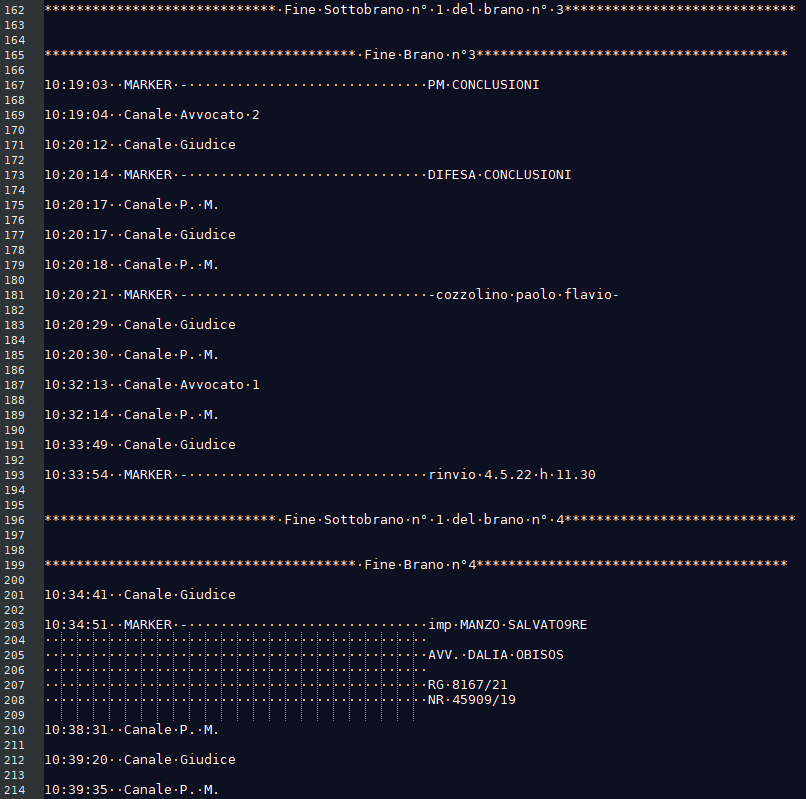
\includegraphics[width=\textwidth,height=12cm]{immagini/file-cronologia.png}
  \caption{Porzione di file cronologia}
\end{figure}
Come possiamo vedere dall'immagine all'interno del file cronologia troviamo i metadati. Nello specifico possiamo vedere in completo il \gls{sottobrano}\glsfirstoccur numero 1 (in questo caso l'unico)
del \gls{brano}\glsfirstoccur numero 4. All'interno di questo sottobrano troviamo i vari \gls{canali}\glsfirstoccur con gli orari in cui in aula sono stati fatti degli interventi, con il nome di riferimento dei canali dedicati
si può facilmente intuire chi abbia preso parola in un dato istante. Inoltre possiamo vedere vari marker che sono gli appunti che il fonico prende nel corso della registrazione e che
interpretati come avviene nella libreria creata appositamente formano i vari procedimenti. Nel caso specifico di questo sottobrano abbiamo una chiusura di un procedimento, come si
può vedere dal marker che dichiara il "rinvio". Scorrendo in giù il nostro file cronologia possiamo vedere come inizi il sottobrano numero 1 del brano numero 5 dove troviamo, grazie al
marker che contiene i codici (RG e RGNR), l'inizio di un nuovo procedimento che continuerà fino ad un nuovo marker di chiusura.
\paragraph{Traccia audio}
E un file mp3 che contiene la registrazione di un canale audio in particolare, che può fare riferimento ad un solo microfono, oppure all'insieme dei microfoni descritto come \gls{traccia mixer}\glsfirstoccur.
Esempio di file all'interno di una cartella:
\begin{figure}[H]
  \centering
  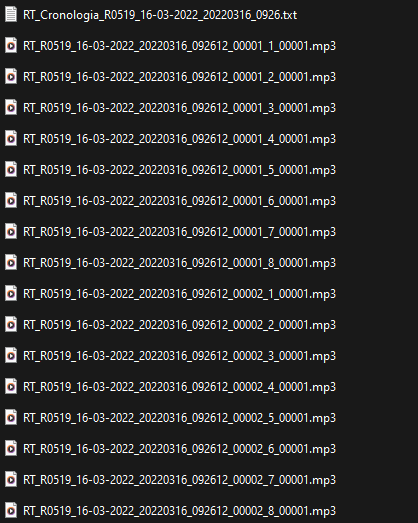
\includegraphics[width=\textwidth,height=12cm]{immagini/CD-files.png}
  \caption{I file all'interno di un CD}
\end{figure}
\begin{itemize}
  \item \verb|RT_Cronologia_R0519_16-03-2022_20220316_0926.txt|: file \textbf{cronologia} che regola tutte le tracce audio presenti nella cartella CD;
  \item \verb|RT_R0519_16-03-2022_20220316_092612_00001_1_00001.mp3|: file audio \textbf{traccia mixer}, contiene la registrazione completa di tutti i microfoni presenti in aula per il Brano 1 e Sottobrano 1;
  \item \verb|RT_R0519_16-03-2022_20220316_092612_00001_2_00001.mp3|: file audio \textbf{giudice}, contiene la registrazione completa del microfono dedicato al giudice per il Brano 1 e Sottobrano 1;
  \item \verb|RT_R0519_16-03-2022_20220316_092612_00001_3_00001.mp3|: file audio \textbf{P.M.}, contiene la registrazione completa del microfono dedicato al Pubblico Ministero per il Brano 1 e Sottobrano 1;
  \item \verb|RT_R0519_16-03-2022_20220316_092612_00001_4_00001.mp3|: file audio \textbf{avvocato 1}, contiene la registrazione completa del microfono dedicato all'avvocato 1 per il Brano 1 e Sottobrano 1;
  \item \verb|RT_R0519_16-03-2022_20220316_092612_00001_5_00001.mp3|: file audio \textbf{avvocato 2}, contiene la registrazione completa del microfono dedicato all'avvocato 2 per il Brano 1 e Sottobrano 1;
  \item \verb|RT_R0519_16-03-2022_20220316_092612_00001_6_00001.mp3|: file audio \textbf{imputato}, contiene la registrazione completa del microfono dedicato all'imputato per il Brano 1 e Sottobrano 1;
  \item \verb|RT_R0519_16-03-2022_20220316_092612_00001_7_00001.mp3|: file audio \textbf{testimone}, contiene la registrazione completa del microfono dedicato al testimone per il Brano 1 e Sottobrano 1;
  \item \verb|RT_R0519_16-03-2022_20220316_092612_00001_8_00001.mp3|: file audio \textbf{ausiliario}, contiene la registrazione completa del microfono ausiliario per il Brano 1 e Sottobrano 1.
\end{itemize}

\subsubsection{Metadati}
I metadati in questo progetto fanno riferimento a ciò che è scritto all'interno del file di cronologia, che viene interpretato dalla libreria appositamente creata per il \gls{parsing}\glsfirstoccur del file.
Questi metadati possono essere di svariati tipi, dipendono dal sistema che li scrive su questo particolare file e dal tecnico che appunta ciò che succede in aula. Di seguito una lista
dei tipi di metadati che sono stati ritenuti rilevanti per l'applicazione e che vengono cercati all'interno del file cronologia per poi essere interpretati:
\begin{itemize}
  \item \textbf{Procedimenti}: questi sono il cuore dei metadati, sono appuntati manualmente dai tecnici e per questo non sempre precisi e presenti. Per ovviare a queste possibilità
        la decisione è stata quella di lasciare la possibilità all'utente di modificarli dopo il caricamento e l'interpretazione da parte della libreria apposita. Il dato più rilevante e
        di interesse per l'applicazione è la combinazione dei due codici \textbf{RG} e \textbf{RGNR} che identifica in modo univoco il procedimento.
  \item \textbf{Interventi}: questi metadati sono di supporto alle registrazioni, e sono automaticamente generati e scritti sul file cronologia dal sistema di registrazione dei file. Come
        facilmente intuibile dal nome scelto per loro riportano gli interventi che sono stati fatti in aula, specificando con delle informazioni da quale microfono e a che ora;
  \item \textbf{Marker}: questi metadati invece non sono generati automaticamente dal sistema ma vengono scritti dai tecnici e inseriti nel file cronologia mediante il sistema di registrazione.
        Essi riportano informazioni di qualsiasi tipo, inizio di un procedimento, fine, parole che magari non si sentono bene in aula o informazioni sui partecipanti alla sessione giudiziaria.
        Vengono riassunti con due campi, uno per l'ora nella quale è stato riportato l'appunto e un altro per la descrizione testuale dell'appunto.
\end{itemize}

%**************************************************************%
\subsection{Libreria per il parsing}
Data la particolare natura dei dati e metadati trattati dall'applicazione si era pensato in sede di analisi e poi di progettazione di realizzare una libreria apposita per
interpretarli. In particolare quello che rendeva indispensabile la creazione di una libreria apposita è la varietà di casi che si possono presentare nei metadati del
file cronologia, in questo file infatti troviamo dei casi abbastanza standard che riguardano gli interventi al microfono dei partecipanti alle udienze, ma troviamo anche
i marker scritti dai fonici mentre l'udienza scorre in aula che assomigliano molto a degli appunti, che possono essere quindi i più disparati possibili, ma che hanno
grande importanza nella nostra applicazione. Questi marker, infatti, contengono delle parole chiave che possono determinare molte cose di grande importanza tra cui
l'inizio di un procedimento, la sua fine, il suo esito e molto altro. Nonostante la grande rilevanza di questi marker per la logica della nostra applicazione,
che si basa interamente su questi metadati, essi sono per la maggior parte scritti manualmente dai tecnici delle aule di tribunale e soggetti quindi ad errori di vario tipo.
La libreria che abbiamo creato prende in input questi metadati caricati dall'utente e dopo una serie di interpretazioni, di vario genere, da in output i dati che l'utente
visualizza all'interno dell'applicazione. Il suo funzionamento si basa su varie funzioni create per l'interpretazione del testo, in particolare per trasformare
il linguaggio naturale (testo scritto dai fonici come i marker) in \gls{oggetti javascript}\glsfirstoccur da poter usare all'interno dell'applicazione. La libreria è divisa in due parti principali,
la prima prende il testo semplice del file cronologia, lo interpreta e ne restituisce una rappresentazione molto complessa, strutturata in oggetti javascript, la seconda
prende questa complessa rappresentazione ad oggetti del file cronologia e la trasforma in \gls{array di oggetti}\glsfirstoccur (appositamente strutturati) da passare allo store Redux. Da
qui i dati saranno disponibili all'interno dell'applicazione per l'utente finale.
\begin{figure}[H]
  \centering
  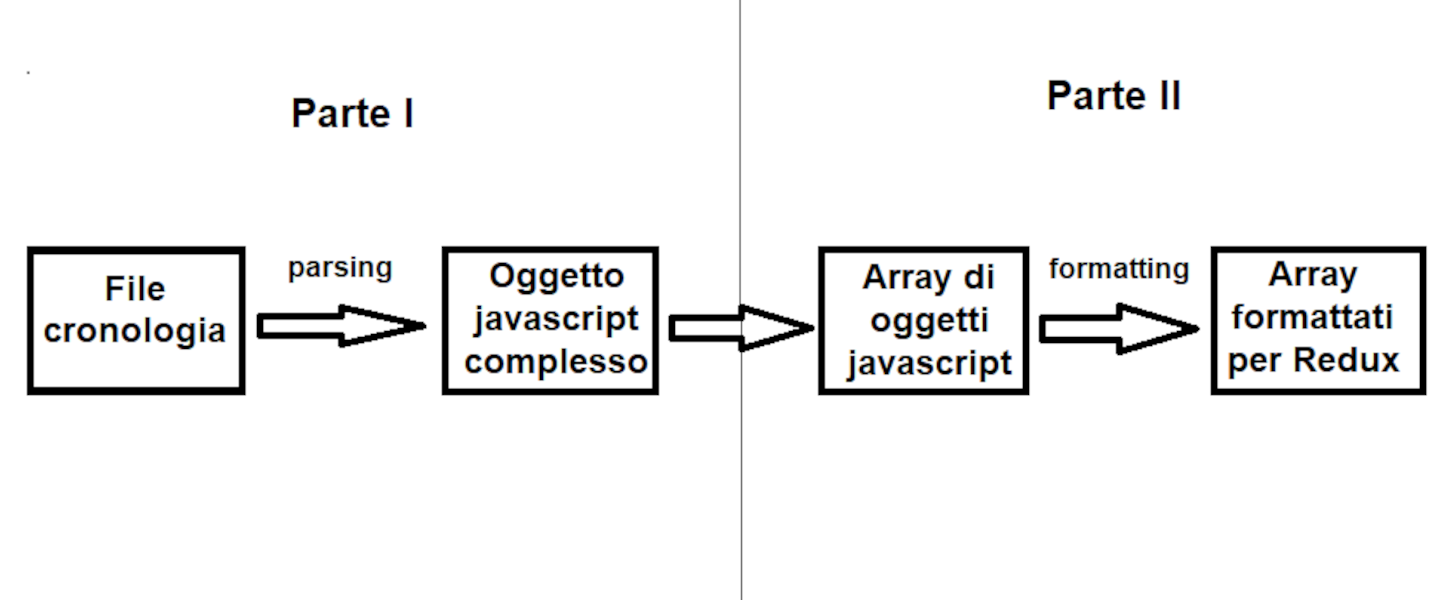
\includegraphics[width=\textwidth]{immagini/libreria-funzionamento.png}
  \caption{Struttura della libreria}
\end{figure}
Di seguito riassumiamo il corso dei dati/metadati e il funzionamento della libreria:
\begin{itemize}
  \item \textbf{input file}: in input la libreria riceve un file cronologia nel formato che abbiamo già visto nel precedente capitolo;
  \item \textbf{parsing del file}: il file viene interpretato e trasformato in un oggetto javascript di struttura complessa (come in figura \ref{fig:libreria-parsing});
  \item \textbf{parsing dell'oggetto}: l'oggetto viene trasformato in una serie di array di oggetti javascript che contengono i metadati del file facilmente utilizzabili
        in qualsiasi applicazione javascript (come in figura \ref{fig:libreria-object});
  \item \textbf{output array}: gli array di oggetti vengono formattati e messi a disposizione per essere caricati e utilizzati nello store Redux che abbiamo scelto come
        gestore dello stato per il lato frontend della nostra applicazione;
\end{itemize}
\begin{figure}[H]
  \centering
  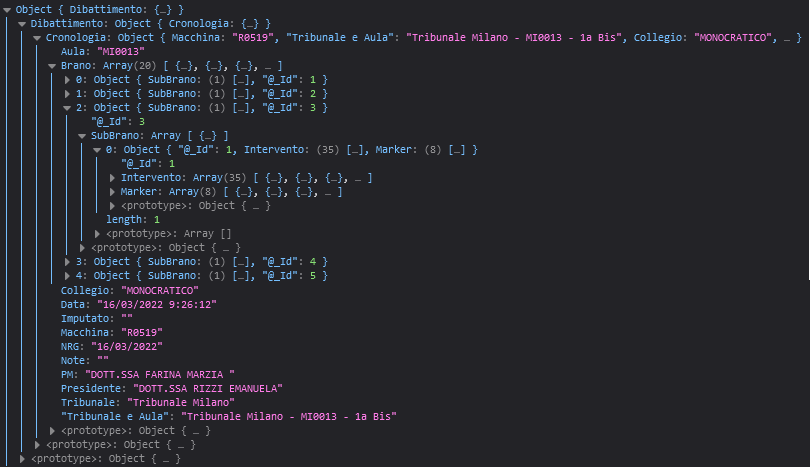
\includegraphics[width=\textwidth]{immagini/libreria-file-parsing.png}
  \caption{L'oggetto javascript risultato dell'interpretazione da parte della libreria del file cronologia}
  \label{fig:libreria-parsing}
\end{figure}
\begin{figure}[H]
  \centering
  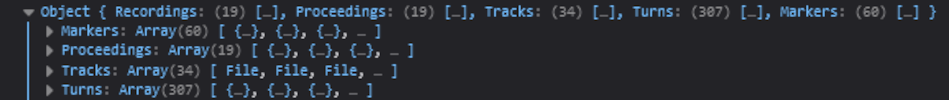
\includegraphics[width=\textwidth]{immagini/libreria-parsing-objects.png}
  \caption{Gli array di oggetti javascript risultato della trasformazione da parte della libreria dell'oggetto in figura \ref{fig:libreria-parsing}}
  \label{fig:libreria-object}
\end{figure}
Difficilmente la libreria sarà riutilizzabile perchè la natura dei dati di input è molto particolare però la sua realizzazione con varie funzioni suddivise in due parti
ben distinte è stata appositamente pensata, per permetterci eventualmente di utilizzare i dati in uscita dalla prima parte dell'interpretazione del file, anche su
un' altra piattaforma che non sia necessariamente la nostra applicazione web scritta in javascript.


%**************************************************************%
\subsection{Redux}
\subsubsection{Store}
Lo store è l'oggetto che contiene tutto lo stato dell'applicazione, viene creato e gestito con Redux e Redux-toolkit ed è completamente separato dalla user interface.
Nel nostro caso questo oggetto è molto complesso, perchè i dati possono diventare numericamente molto grandi in modo veloce e perchè la loro rappresentazione in alcuni casi può
essere non serializzata, cioè dati non standard, come Redux prevede. Per ovviare a questo inconveniente che è stato riscontrato per tutte le operazioni che coinvolgono i dati di tipo File,
centrali nello sviluppo del nostro frontend, abbiamo sfruttato la possibilità che da Redux di disabilitare il controllo sulla serializzazione per alcuni dati. Con le funzioni che Redux mette a disposizione
la creazione e la manutenzione dello store risulta molto facile, una volta che è stato compreso come questo si comporta. Lo store rappresenta per la nostra applicazione lato frontend
il punto dove vengono mantenuti tutti i dati e le operazioni che possono essere eseguite su questi. Lo store, infatti, non rappresenta solo un modello di dati ma un vero e proprio stato dell'applicazione,
cioè un insieme di dati e azioni che in un dato momento è possibile compiere. Per facilitare l'implementazione ma soprattutto la manutenzione del codice lo store può essere diviso in
\textbf{slice}, ovvero fette di dati, nel nostro caso abbiamo suddiviso lo store in due slice principali, una riguardante i dati caricati dall'utente e un altra con le operazioni che
coinvolgono chiamate alle API. La caratteristica principale di uno store Redux e di come questo strumento gestisca lo stato dell'applicazione è che i dati all'interno dello store sono
immutabili, cioè non possono essere cambiati o sovrascritti direttamente ma bisogna sempre passare per le apposite funzioni chiamate \textbf{action} che Redux permette di creare per implementare
il modo di cambiare lo stato. Queste action sono la regola per gestire lo stato con Redux perchè lavorando in questo modo si permette a questo strumento di avere sempre il controllo dello stato ad ogni modifica
e in particolare di ricalcolare lo stato solo nella misura in cui una action prevede. Questo nuovo stato viene poi aggiornato automaticamente nei componenti React dopo il ricalcolo.
Tutte le nostre action sono create all'interno di particolari funzioni della libreria Redux chiamate \textbf{reducer} che ricevono come parametri lo stato e l'azione e permettono il
calcolo del nuovo stato. Ogni reducer può essere richiamato all'interno dell'applicazione con il metodo Redux \textbf{dispatch} che scatena l'azione di riferimento sullo stato attuale.
Infine per rendere disponibili i dati presenti nello store si possono creare dei \textbf{selector} che selezionano porzioni di dati dallo store e le rendono disponibili nei componenti React.

\subsubsection{Creazione dello Store}
Lo store implementato con Redux, viene creato in un apposito file javascript all'esterno dell'applicazione React, in modo da mantenere la separazione, e viene passato all'applicazione
in un unico punto, che per convenzione è il file index.jsx dove tutta l'applicazione risiede. Lo store viene creato con un particolare metodo di Redux che ha la funzione di combinare
tutte le slice che abbiamo creato ma non solo, permette di definire anche casi particolari, infatti è proprio in questa fase di creazione dello store che abbiamo "richiesto" a Redux di non
verificare la serializzazione di alcuni dati, come spiegato in precedenza.

\begin{figure}[H]
  \centering
  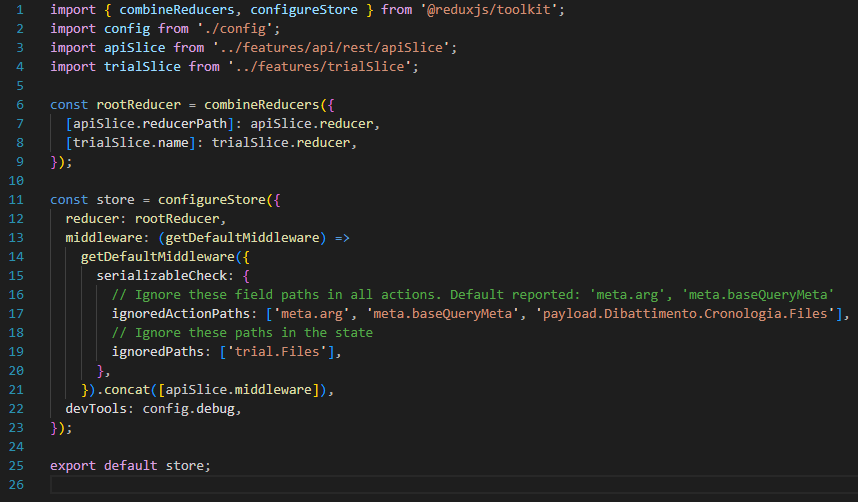
\includegraphics[width=\textwidth]{immagini/creazione-store.png}
  \caption{Creazione dello store dell'applicazione}
\end{figure}

\subsubsection{Slice e Reducer}
Una slice contiene una parte del nostro store, nel caso della nostra apllicazione si è deciso di dividere lo store in due slice una per la parte dove vengono salvati i dati da
visualizzare e modificare all'interno dell'applicazione (procedimenti, registrazioni e tracce) e l'altra per la parte che gestisce le richieste tramite API al backend, per questa
seconda slice è necessario l'utilizzo della libreria Redux-toolkit che ha una serie di funzioni che permette di facilitare le richieste, e di integrare le risposte direttamente nello store.
Ogni slice ha i propri reducer, ovvero le funzioni che prendendo in input lo stato attuale e una action e restituiscono il nuovo stato modificato secondo quello che l'azione prevede.
Nel nostro caso per mantenere più ordinata possibile la gestione dello stato ogni slice presenta il proprio reducer che contiene le varie action.

\begin{figure}[H]
  \centering
  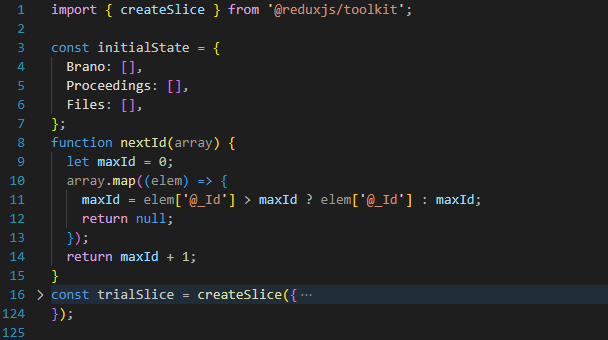
\includegraphics[width=\textwidth]{immagini/slice-reducer.png}
  \caption{Slice che rappresenta i nostri dati all'interno dell'applicazione}
\end{figure}

\subsubsection{Action}
Le action modificano lo stato dell'applicazione senza farlo direttamente ma demandando la vera e propria modifica dei dati a Redux. I dati come accennato in precedenza sono immutabili
quando si implementa uno store con Redux per la gestione dello stato di un applicazione, questo significa che operazioni come arrayDiDati[chiave] = valore non sono possibili
direttamente dal codice. Per mantenere lo stato logicamente corretto, efficente e valido i dati vanno modificati creando delle action, che prevedono il passaggio dello stato attuale
e dei paramentri aggiuntivi come input e restituiscono un nuovo stato dell'applicazione.

\begin{figure}[H]
  \centering
  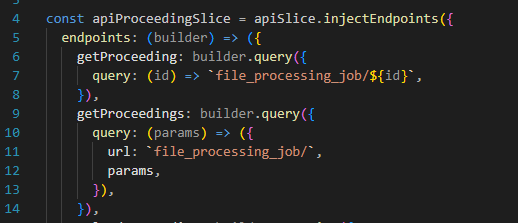
\includegraphics[width=\textwidth]{immagini/api-action.png}
  \caption{Actions con chiamate al backend}
\end{figure}

\subsubsection{Selector}
Per reperire una porzione di dati come per esempio un array di registrazioni o un singolo procedimento all'interno del nostro store abbiamo bisogno dei selector, questi sono delle
piccole funzioni che fanno un'azione di filtro sull'intero store restituendo solo quello che abbiamo richiesto. La vera funzione di un selector oltre a filtrare lo store è quella di
mantenere questo filtro attivo sempre all'interno dell'applicazione finchè non cambia lo stato, infatti i dati selezionati con un selector, vengono ricalcolati soltanto se una
modifica allo store (tramite action) coinvolge almeno uno dei dati stessi.

\begin{figure}[H]
  \centering
  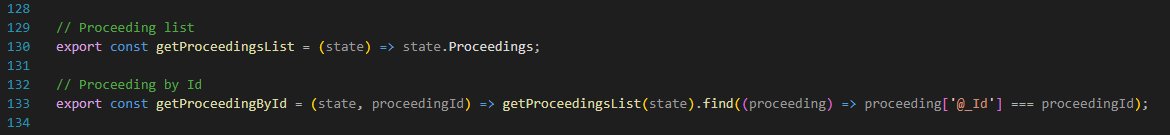
\includegraphics[width=\textwidth,height=3cm]{immagini/selectors.png}
  \caption{Selectors per selezionare i procedimenti dallo store}
\end{figure}

%**************************************************************%
\subsection{React}

\subsubsection{Component}
La scelta di react in fase di analisi del progetto ci permette di utilizzare i component tipici di questa libreria javascript. Il concetto di component è molto intuitivo quando ci si
approccia ad usare React, essi sono come delle funzioni javascript che accettano in input dei particolari parametri chiamati \textbf{props}, e ritornano elementi React che
descrivono cosa si dovrà vedere sullo schermo. Usando i components possiamo facilmente dividere la user interface in piccole parti indipendenti tra loro e riusabili, in modo da
doverci occupare di una parte alla volta pensando solo a quella in modo isolato prima di integrarla con il resto della UI.
I component secondo React possono essere di due tipi class component o function component, nel nostro caso abbiamo scelto di costruire tutti function component principalmente
per avere un codice più leggibile e perchè non c'è la necessità di avere i vantaggi dei class component (in particolare non ci serve nessun metodo costruttore all'interno dei component
che abbiamo creato). I component possono quindi essere una qualsiasi parte della user interface che vogliamo realizzare, da un bottone a un form oppure un intera vista. Sviluppando la
nostra applicazione abbiamo pensato inizialmente ai component più "esterni", cioè quelli che fanno da contenitore agli altri, andando poi a raffinare sempre di più fino ai component
più "interni", ossia quelli riguardanti le parti più piccole dell'applicazione, usando in questo modo una sorta di metodo top-down per lo sviluppo delle componenti necessarie.
Una vola che abbiamo creato i vari component, utilizzando questo modello top-down, siamo passati all'integrazione. React permette molto agevolmente, proprio come punto di forza
nell'uso di questa libreria, l'integrazione tra i vari componenti. Basta importare nella pagina il componente che ci serve, richiamarlo nel codice come se fosse un normale tag
HTML e passargli le props di cui ha bisogno, non dobbiamo preoccuparci di altro, React svolgerà per noi il corretto rendering dell'insieme dei componenti.

\begin{figure}[H]
  \centering
  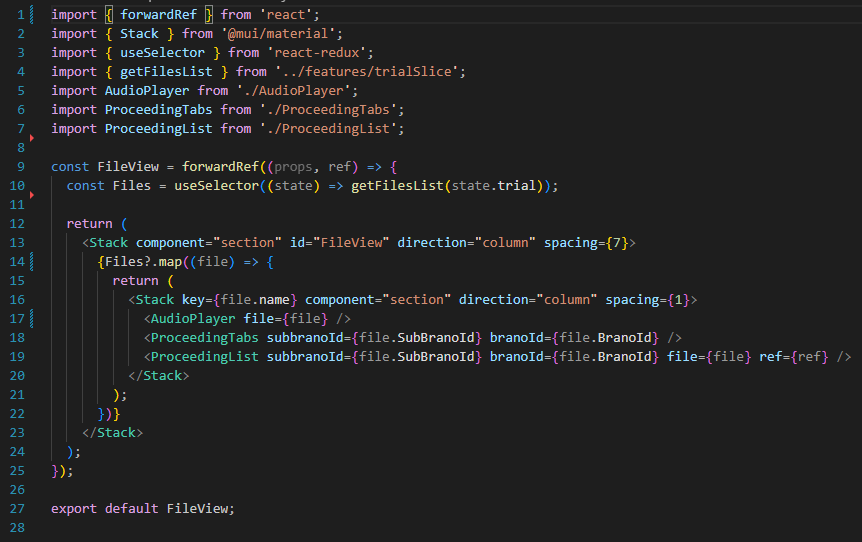
\includegraphics[width=\textwidth]{immagini/fileView-component.png}
  \caption{Codice del component fileView per la vista dei file caricati}
\end{figure}

Vediamo nel dettaglio come viene reralizzato un component nella nostra applicazione, nello specifico il component fileView, che realizza un intera vista occupandosi di visualizzare
la lista di tutti i file dopo che sono stati caricati dall'utente.
Questo componente non necessita di alcuna props ma si serve di uno dei selector Redux che abbiamo creato per reperire la lista dei file di cui abbiamo bisogno dallo store. (riga 10)
La lista dei file recuperata grazie all'apposito selector viene snocciolata con la funzione nativa javascript map (riga 14), che permette di eseguire delle operazioni per ogni
oggetto della lista, nel nostro caso per ogni file. In questo component per ogni file si desidera richiamare altri tre component che si occuperanno di alcune parti
della user interface che riguarda ogni file, e sono:
\begin{itemize}
  \item \textbf{AudioPlayer}: che provvede a fare il render di un player per riprodurre il file;
  \item \textbf{ProceedingTabs}: tramite una tendina permette di visualizzare e gestire i metadati relativi al file (Marker e Interventi);
  \item \textbf{ProceedingList}: recupera e visualizza tutti i procedimenti relativi a questo file.
\end{itemize}

\newpage

\begin{figure}[H]
  \centering
  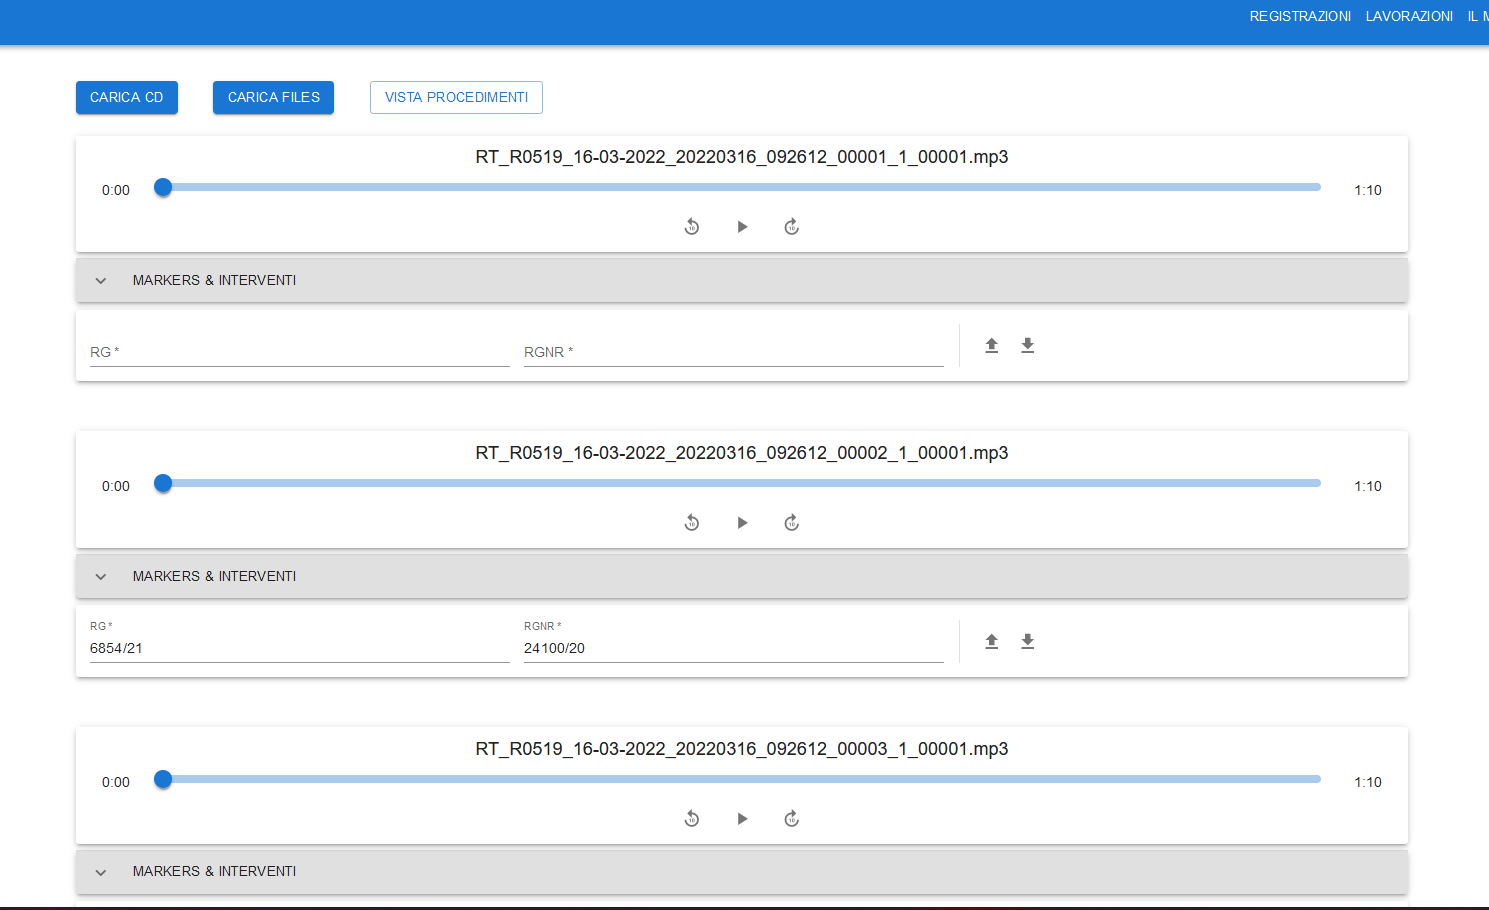
\includegraphics[width=\textwidth,height=12cm]{immagini/fileView-render.png}
  \caption{Render grafico del component fileView per la vista dei file caricati}
\end{figure}

\subsubsection{Hooks}
Gli Hook sono delle funzioni javascript che permettono di entrare nel ciclo usato da React per renderizzare i componenti, e in questo modo descriverne il comportamento.
Queste funzioni non possono essere usate nei componenti di tipo classe e hanno delle regole di invocazione abbastanza rigide, per proteggere lo stato dell'applicazione e il
ciclo di rendering. Gli hook infatti non possono essere chiamati all'interno di cicli, istruzioni condizionali o funzioni che non siano componenti react. La libreria React mette
a disposizione degli Hook generici che risultano molto utili per gestire il rendering dei componenti, ma se questi non dovessero bastare possiamo anche crearne di personalizzati.
Di seguito vediamo un hook appositamente creato per recuperare dal backend la lista dei jobs, è stato creato per essere riusato qualora si rendesse necessario da un altra parte
dell'applicazione ma anche perchè sfruttando le proprietà del linguaggio e in particolare di queste speciali funzioni possiamo facilmente gestire il filtraggio e la
paginazione della lista dei jobs.

\begin{figure}[H]
  \centering
  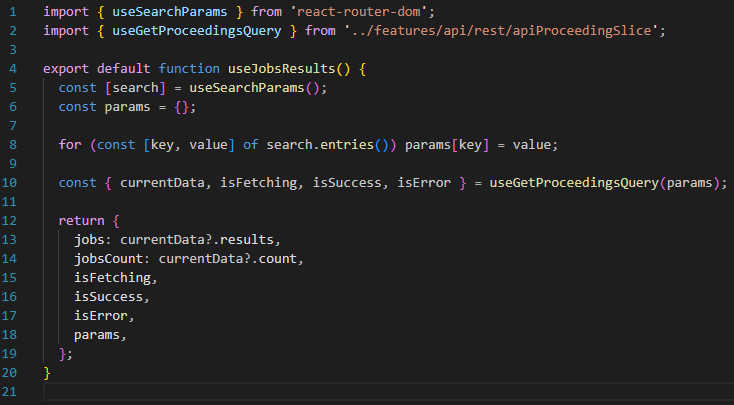
\includegraphics[width=\textwidth]{immagini/useJobResult-hook.png}
  \caption{Codice del hook creato per la visualizzazione dei procedimenti caricati}
\end{figure}

% \subsubsection{Routing}
% [[[[Ha senso questa sezione???]]]]
\subsection{MUI}
\subsubsection{UI style}
Lo sviluppo della parte grafica, in particolare per quanto riguarda lo stile dell'applicazione, non aveva nessun vincolo, si è scelta una soluzione che possa essere intuitiva,
veloce da implementare e generalmente riconosciuta. La scelta fatta è stata l'utilizzo di \textbf{MUI - Material UI} che è una libreria open-source di componenti React già precostruiti
seguendo le regolole di Google Material Design. Material è un sistema di design creato da Google per velocizzare lo sviluppo dei componenti. MUI permette di non doversi preoccupare
di aspetti chiave quali responsive-design, integrazione grafica dei nuovi componenti, stile generale dell'applicazione, perchè tutti questi aspetti vengono automatizzati usando
stili globali e appunto componenti già preimpostati, semplicemente da configurare in base alle necessità.

\begin{figure}[H]
  \centering
  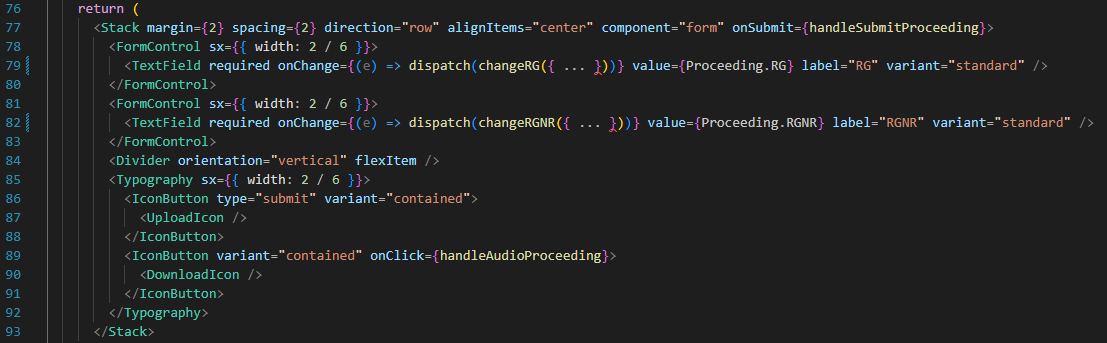
\includegraphics[width=\textwidth, height=8cm]{immagini/proceedingCard-MUI.png}
  \caption{Codice del componente per visualizzare un procedimento}
\end{figure}

In questo esempio preso direttamente da uno dei componenti della nostra applicazione, possiamo vedere vari MUI component utilizzati e personalizzati appositamente per il
nostro funzionamento. Tra questi c'è per esempio \textbf{<Stack>} che costruisce una pila di sottocomponenti, che possono essere direzionati in colonna o in riga (come nel nostro caso).
Altri utilizzi sono \textbf{<FormControl>} e \textbf{<TextField>} che costruiscono una porzione di un form con un campo di tipo testo al suo interno.

\begin{figure}[H]
  \centering
  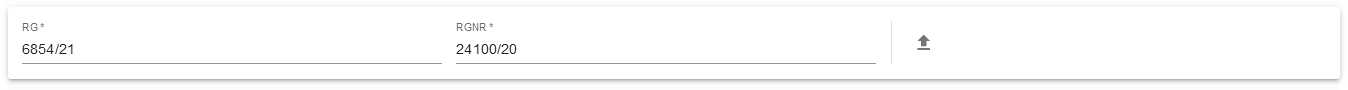
\includegraphics[width=\textwidth, height=2cm]{immagini/proceedingCard-render.png}
  \caption{Render grafico del componente per visualizzare un procedimento}
\end{figure}

\newpage
%**************************************************************%
%**************************************************************%
%**************************************************************%
\section{Testing}
Parte importante del nostro processo di sviluppo, sono i test. Secondo regola aziendale ma anche seguendo il piano di progetto dello stage è stata pianificata una buona parte di ore di testing. Le ore di
testing sono state ripartite in modo proporzionale alle ore di sviluppo di ogni funzionalità. Nella fase iniziale di studio delle tecnologie da utilizzare per il progetto sono state incluse anche varie librerie per
i test su funzioni javascript e componenti React che sono la grande parte del prodotto da realizzare. Dopo un confronto con il tutor si è deciso di intraprendere la strada di \textbf{React-testing-library}\footcite{site:rtl} per il testing dei componenti
e appoggiarci a \textbf{jest}\footcite{site:jest} per la parte javascript dei test.

%**************************************************************%
\subsection{Test javascript function}
Il framework jest è uno dei più diffusi per il test di applicazioni javascript, è focalizzato sulla semplicità nella scrittura dei test e risulta comunque in grado di testare tutte le parti di nostro interesse.
All'interno dei nostri test è stato usato in supporto a React-testing-library per il testing dei componenti React e in prima battuta per il test di tutte le utility javascript che abbiamo creato, in particolare si è reso molto importante
nel testing delle funzioni che leggono i metadati caricati dall'utente e li manipolano per renderli usabili nell'applicazione. Il funzionamento di jest è molto semplice per i nostri casi, ma può essere esteso a molti altri
tipi di test. Per noi è semplice e molto intuitivo creare un test javascript con questo framework, basta creare le condizioni per l'utilizzo di una determinata funzione che vogliamo testare, chimarla come se
dovessimo realmente utilizzarla e vedere se i risultati in usicta da questa chiamata sono quelli che ci aspettiamo.

\begin{figure}[H]
  \centering
  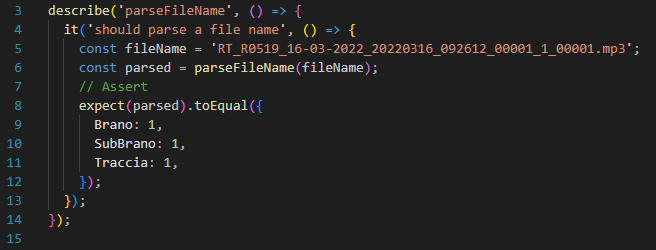
\includegraphics[width=\textwidth]{immagini/test-cronologia.png}
  \caption{Codice del test per una funzione javascript}
\end{figure}

Nella prima parte del test come si può vedere abbiamo creato i dati fittizzi (fileName riga 5) che ci servono da passare alla funzione da testare (in questo caso parseFileName riga 6), in seguito abbiamo effettuato la chiamata di funzione e
per concludere il test abbiamo scritto delle particolari funzioni (expect, toEqual riga 9) con le quali andare a vedere se i risultati ottenuti sono quelli che ci aspettiamo passando i nostri dati fittizzi.

%**************************************************************%
\subsection{Test React component}
La libreria usata è React-testing-library, questa si appoggia completamente su un altra libreria di testing chiamata DOM-testing-library e fornisce una abbastanza completa suite di testing per i componenti React.
% [[[Prima devo dire che si basa sul testare il DOM]]]
Il principio che guida questa libreria e anche i nostri test sui componenti è che i test di integrazione hanno maggior valore degli unit test nel caso di applicazioni React. In particolare con queste librerie (React-testing e jest) usate in modo combinato
si creano test su parti di applicazione dopo il rendering, ovvero la logica dei nostri test è quella di andare a verificare funzionamenti e presenza di elementi nel DOM dopo che è stato fatto il rendering
dell'applicazione. Questo tipo di test ovviamente è un test di integrazione in quanto non va a testare singolarmente ogni componente e ogni funzionalità del componente ma esegue un test della UI dal punto di vista dell'utente, cioè controlliamo che
l'applicazione in ogni momento si comporti come abbiamo progettato che lo faccia.
La libreria prevede di descrivere un test passando ad un apposito metodo il componente di cui fare il render, e una volta che questo è stato completato con altri metodi specifici si va a controllare cosa è nel DOM. Altre situazioni
possono esssere sottoposte a test in questo modo, come scatenare in modo controllato un evento (per esempio il click su un bottone) e vedere se il DOM si modifica come ci si aspetta. Ci sono molte altre possibilità per
casi più particolari come per testare chiamate ad API, nella nostra applicazione però questo tipo di test non è stato implementato per motivi di tempo e in accordo con l'azienda che prevede di mettere appunto
una specifica suite di test per questo ambito per vari prodotti che segue.

\begin{figure}[H]
  \centering
  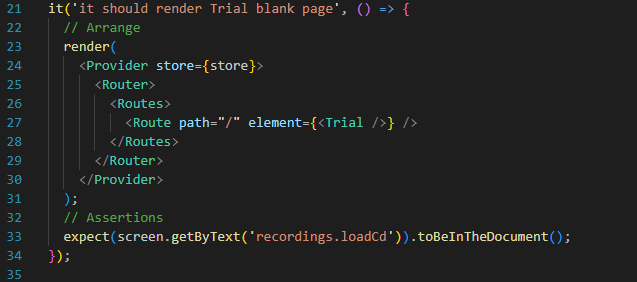
\includegraphics[width=\textwidth]{immagini/test-trial.png}
  \caption{Codice del test per un componente React}
\end{figure}

Nel nostro piccolo esempio che abbiamo riportato qui di test di un componente si può vedere come sia facile e veloce implementare un test di questo tipo, ma allo stesso tempo come
verifichi esattamente quello che ci aspettiamo dalla nostra applicazione. In questo caso dopo il rendering del nostro componente testato (Trial) andiamo a controllare
se nel DOM sono presenti gli elementi che ci aspettiamo, in questo caso un semplice bottone con testo preso dal file delle traduzioni (recordings.loadCD).

%**************************************************************%
% \subsection{Test Redux store}
% Come suggerisce la libreria Redux non c'è un vero e proprio modo di testare in isolamento lo store piuttosto che le action o i selector, il sugerimento è in linea generale quello React standard e cioè testare l'applicazione nel suo complesso, in particolare preferire integration test a unit test.
% Per quanto riguarda la nostra applicazione quindi non abbiamo scritto particolari test per lo store gestito tramite Redux ma ci siamo limitati a verificare tramite i test di integrazione React a verificare il funzionamento dello store stesso.
%   [[[[tengo???]]]]